\part{\LaTeX{} Miscellany}

\section{Tables}
\begin{itemize}
\item We can create tabular content in a \LaTeX{} document either within
  a float environment or not. We will describe what a float is in a moment.

\item Either way, tabular content like the following is created with
  the \texttt{tabular} environment.

\begin{center}
  \begin{tabular}{c c c}
    \hline
    \hline
    State             & Capital    & State Bird             \\
    \hline
    New Jersey        & Trenton    & Eastern Goldfinch      \\
    Connecticut       & Hartford   & American Robin         \\
    New York          & Albany     & Eastern Bluebird       \\
    Massachusetts     & Boston     & Black-capped Chickadee \\
    \hline
    \hline
  \end{tabular}
\end{center}


\item The \texttt{tabular} environment takes a mandatory argument that is
  enclosed in curly braces. In the case of the above table where each column is
  center justified, we'd use \verb! \begin{tabular}{c c c} \end{tabular}!. If we
  wanted the columns to be right-justified or left-justified we could use
  \texttt{r} or \texttt{l} in place of the three \verb=c='s.

\item If we wanted to add a vertical line on either the left or right or in-between two columns we'd use the  argument \verb!{| c | c | c |}!.

\item Horizontal lines are given by \verb!\hline!.

\item Tab breaks are caused by \verb!&! and line breaks by \verb!\\!.

\item The full code for the above table is:\\
  \lstinputlisting{./chapters/05_misc/table.tex}

\item There are much more complex environments than \texttt{tabular} that you
  will have to use once your tabular content grows. They are similar, but have
  their own documentation to help you through.

\end{itemize}

\section{Pictures}

\begin{itemize}

\item \LaTeX{} has the ability to draw arbitrary types of objects and schematics
  within a \LaTeX{} document in a native language. However, this is sometimes
  overkill. If necessary, you can learn about this later.

\item Download \texttt{Image1.pdf} and \texttt{Image2.png} from
  \url{www.rochester.edu/college/gradstudents/jolmsted/}

\item In your preamble, add the \texttt{graphicx} package (i.e.\
  \verb!\usepackage{graphicx}!)

\item Where you'd like the picture to show up, type
  \verb!\includegraphics{./Image1}! without a file extension and be
  sure to use the appropriate path to the image file, relative to the
  \LaTeX{} document. The file extension is not necessary.
\item The \verb!scale! optional argument is useful to change
  dimensions on the fly without distorting the aspect ratio.
\item Try the following code in a \LaTeX{} document environment:

  \ovalbox{
    \begin{minipage}{\linewidth}
\begin{verbatim}

  \begin{center}
    \fbox{
      \fbox{
        \includegraphics[scale=.25]{./extra/Image1}
      }
      \fbox{
        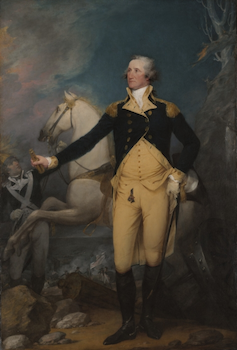
\includegraphics[width=3in,
        height=1in,
        angle=90]{./extra/Image2}
      }
    }
  \end{center}

\end{verbatim}
    \end{minipage}
  }

\item The result is something like
  \begin{center}
    \fbox{
      \fbox{
        \includegraphics[scale=.25]{./extra/Image1}
      }
      \fbox{
        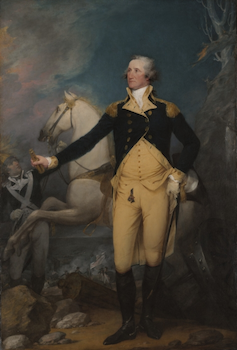
\includegraphics[width=3in,
        height=1in,
        angle=90]{./extra/Image2}
      }
    }
  \end{center}

\item Notice that we didn't have to specify the file extension. Notice
  the order in which the \texttt{angle} and then
  \texttt{height}/\texttt{width} arguments are applied. What does
  \verb!\fbox{}! do?


\end{itemize}

\section{Floats}
\begin{itemize}
\item Although we can create tables with the \texttt{tabular}
  environment and we use \verb!\includegraphics{}! to insert external
  image files, these commands are seldom placed inside a document
  without entering them in a special environment.
\item Typically, these kinds of content are placed in \textit{floats}
  which act like containers for tables and figures. \LaTeX{},
  according to a set of rules, figures where these containers should
  be placed which depends on the content before the float, the content
  after the float, and the \LaTeX{} code within the float.

\item If nothing else, the big adjustment required by users placing
  content in floats is realizing that the placement of a table or
  figure is up to \LaTeX{} and
  ``jury-rigging''/''jimmy-rigging''/''jerry-rigging'' the placement
  is ill-advised.

\item The float for tables is
  \verb!\begin{table}[htpb] \end{table}!. The optional \verb![thpb]!
  argument provides \LaTeX with some instructions on where to place
  the table.

\item The float environment for figures is
  \verb!\begin{figure}[htpb] \end{figure}!. Notice, again, the
  optional argument.

\item In actuality, there need not be anything inside these float
  environments, or it could easily be regular \LaTeX{} markup.

\item \verb!\caption{}!, placed somewhere in the float, allows a title
  of the content to be placed and automatically numbered.

\item \verb!\label{}!, placed immediately after the \verb!\caption{}!
  command gives an identified to the object by which it can be
  referred for directing readers to Figure 1 or Table 4 without
  hard-coding the float order.

\item Try: \\
  \ovalbox{
    \begin{minipage}{\linewidth}
\begin{verbatim}
\begin{figure}
  \begin{center}
    \fbox{
      \includegraphics[width=3in,
      height=1in,
      angle=120]{./Image2}
    }
    \caption{A Hero of a Man} \label{f:Riker}
  \end{center}
\end{figure}
\end{verbatim}
    \end{minipage}
  }

\item Now, see Figure \ref{f:Riker} on page \pageref{f:Riker} to view the
  output. We were able to reference the figure number automatically using
  \verb!\ref{f:Riker}! which matches our \verb!\label!. We reference the page
  number automatically with \verb!\pageref{}!.
  \\

\begin{figure}
  \begin{center}
    \fbox{
      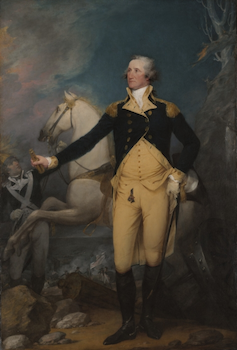
\includegraphics[width=3in,height=1in,angle=120]{./extra/Image2}
    }
    \caption{A Hero of a Man} \label{f:Riker}
  \end{center}
\end{figure}

\end{itemize}

\section*{More Math Environments}
\begin{itemize}
\item There are a number of math environments that become useful when
  one is typesetting mathematical notation beyond very basic
  experessions.
\item As in a previous tutorial, add
  \verb!\usepackage{amsmath, amsthm, amssymb, amsfonts}! to the
  preamble if not already there.
\end{itemize}

\subsection*{Fraction}
There are instances where $3/4$ would look better as $\frac{3}{4}$ and
this works equally well for longer expressions $$
\frac{\tan\left(\cos\left(\sin (X) \right)\right)}{\int_{\mathbb{R}}
  f(x) ~ dx}.$$ It is the command \verb!\frac{}{}! which provides
this. The numerator is the first argument and the denominator is the
second.
\subsection*{Equation}
The equation environment is a very common way to typeset equations
when reference numbers are being used. So, for example,
\verb!\begin{equation} 4=x^2 \end{equation}! gives
\begin{equation}
  4=x^2.
\end{equation}
Now, it is not necessary to place the equation environment in a math
mode. In this sense, the math mode is implied. There is also a variant
such that \verb!\begin{equation*} 4=x^2 \end{equation*}! suppresses
the equation numbering,
\begin{equation*}
  4=x^2.
\end{equation*}
Equation numbers can be labeled and referenced as was done in the
figure environment. This is a single equation environment and if you
try to enter line breaks such that you could force another line, it
will fail. In that case, I find the \texttt{align} approach being the
easiest because it is flexible.

\subsection*{Align}
The \texttt{align} environment allows you to enter multiple lines and
include alignment stops. There is a un-numbered version,
\texttt{align*}, too. The code

\ovalbox{
    \begin{minipage}{\linewidth}
\begin{verbatim}
\begin{align}
   \sum_{x=1}^{4} \frac{1}{x} &
   &= \frac{1}{1} + \frac{1}{2}  + \frac{1}{3} + \frac{1}{4} & \\
   &= \frac{25}{12} &\\
   & &>2
\end{align}
\end{verbatim}
    \end{minipage}
  }
produces a three line \texttt{align} environment.
\begin{align}
   \sum_{x=1}^{4} \frac{1}{x}
   &= \frac{1}{1} + \frac{1}{2}  + \frac{1}{3} + \frac{1}{4} \\
   &= \frac{25}{12} \\
   &>2
\end{align}
Notice that the numbering is cumulative. The use of \verb!\label{}!
and \verb!ref{}! works identically here.


\subsection*{Array}
The \texttt{array} environment provides a unified way of representing
vectors and matrices. The environment begins in the standard
\verb!\begin{array}{cc} \end{array}! way, but the mandatory
\verb!{cc}! argument specifies there are two center-justified
columns. Changes to this argument proceed identically to the argument
in the creation of tables. On important point is that the array
environment does not create its own math mode environment, so we must
put it inside one when we use it. We get \[ \left[\begin{array}{cc} 1 & 0 \\
    0 & 1\end{array}\right], \] the two dimensional identity matrix
from \\
\ovalbox{
    \begin{minipage}{\linewidth}
\begin{verbatim}
\[
 \left[
\begin{array}{cc}
  1 & 0 \\
  0 & 1
\end{array}
\right],
\]
\end{verbatim}
    \end{minipage}
  } \\ Notice the comma in the source code. It must be in the display
  math environment so that it is placed adjacent to the matrix and not
  in the text. By changing the number of rows, columns, and the
  delimiters, most matrix-like objects can be represented with this
  environment.

\subsection*{Cases}

The \texttt{cases} environment is both extremely useful, but quite
narrow in application. Although it is designed to be used only to
represent piece-wise functions, it is a marked improvement over the
alternative which would be to ``hack'' the \texttt{array}
environment. Like the \texttt{array} environment, though,
\texttt{cases} must be used within math mode. So,

\[
\mathbf{1}_{\mathcal{X}}(x) =
\begin{cases}
  1, & x \in \mathcal{X} \\
  0, & \textrm{otherwise}
\end{cases}
\]
is the result of the code

\ovalbox{
    \begin{minipage}{\linewidth}
\begin{verbatim}
\[
\mathbf{1}_{\mathcal{X}}(x) =
\begin{cases}
  1, & x \in \mathcal{X} \\
  0, & \textrm{otherwise}
\end{cases}.
\]
\end{verbatim}
    \end{minipage}
  } Notice how I use whitespace and line breaks to organize the code
  although \LaTeX{} won't interpret it.

\section{Words of Wisdom}

\begin{itemize}
\item It is considered good practice to keep text file contents within
  the first 80 characters. This may seem weird or hard, but this,
  along with use of the \texttt{\%} and comments will make the input
      file more human-readable.
    \item As you learn \LaTeX{} don't worry about trying to make
      \LaTeX{} look a certain way. Tell \LaTeX{} about your content
      and its structure. Let \LaTeX{} worry about the details of
      appearance.
    \item Google is your friend.

    \item Comment out error-laden parts of code. Add things back in
      one at a time until you've identified the source of your
      syntactical mistakes.

    \item Let WinEdt help you. It highlights the source file according
      to rules. If the rules are broken, the highlighting will appear
      other it should and this is a visual cue that something is
      wrong.

    \item Because \LaTeX{} seldom interprets whitespace in too
      generous a way, use it as an organizational tool.
\end{itemize}


%%% Local Variables:
%%% mode: latex
%%% TeX-master: "../../tutorial"
%%% End: